\documentclass[paper=a4,DIV=12]{leetcode}

\usepackage[T1]{fontenc}
\usepackage[utf8]{inputenc}
\usepackage{courier}
\usepackage{tgtermes,newtxtext,newtxmath}
\usepackage[pdftex,colorlinks,allcolors=blue]{hyperref}
\usepackage{natbib}

\usepackage{amsmath,amsfonts}
\usepackage{tikz}
\usetikzlibrary{arrows,3d,patterns,calc}

\setcitestyle{numbers,square,comma}

\begin{document}

\serietitle{LeetCode contests solutions}
\title{1793. Building Boxes~\cite{leetcode:1739}}
\subtitle{}
\author{Paweł Tomulik}
\date{2024-06-15}
\maketitle

\section{Description}
\label{sec:description}

You have a cubic storeroom where the width, length, and height of the room are
all equal to $n$ units. You are asked to place $n$ boxes in this room where
each box is a cube of unit side length. There are however some rules to placing
the boxes:

\begin{itemize}
  \item You can place the boxes anywhere on the floor. If box $x$ is placed on
    top of the box $y$, then each side of the four vertical sides of the box
    $y$ must either be adjacent to another box or to a wall.

  \item Given an integer $n$, return the minimum possible number $f$ of boxes
    touching the {\em floor}.
\end{itemize}

\section{Solution}
\label{sec:solution}

\subsection{Complexity}
\label{sec:complexity}

Solvable in $\mathcal{O}(1)$.

\subsection{Solution description}
\label{sec:solution-description}

To minimize the ``floor cost'', we must put as much boxes as possible on top of
other boxes (base boxes). To provide required surroundings for the base boxes
at minimal ``floor cost'', we have to utilize walls to the maximum extent
possible. Concluding -- we shall build a~``pyramid'' in a~corner.

An~``ideal pyramid'' of size $k$ is actually a~box version of a~ball
tetrahedron with $k$ boxes along each edge. Figure~\ref{fig:7YP7N} depicts
an~``ideal pyramid'' of size $4$. The total number of boxes in that
tetrahedron is given by $k$'th tetrahedral number~\cite{enwiki:1226358199}
%%%%%%%%%%%%%%%%%%%%%%%%%%%%%%%%%%%%%%%%%%%%%%%%%%%%%%%%%%%%%%%%%%%%%%%%%%%%%%
\begin{equation}
  Th(k) = \frac{k(k+1)(k+2)}{6}.
  \label{eq:BP9CM}
\end{equation}
%%%%%%%%%%%%%%%%%%%%%%%%%%%%%%%%%%%%%%%%%%%%%%%%%%%%%%%%%%%%%%%%%%%%%%%%%%%%%%
%%%%%%%%%%%%%%%%%%%%%%%%%%%%%%%%%%%%%%%%%%%%%%%%%%%%%%%%%%%%%%%%%%%%%%%%%%%%%%
\begin{figure}[htbp]
  \centering
  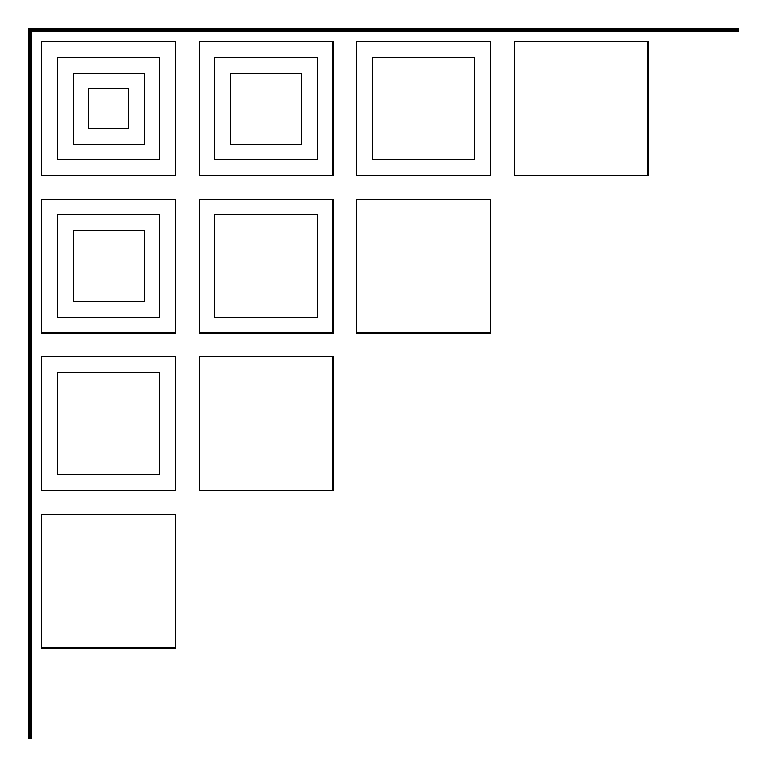
\begin{tikzpicture}[]
    \foreach \k [evaluate=\k as \s using {0.25+0.20*\k}] in {3, ..., 0} {
      \foreach \i [evaluate=\i as \m using {\k-\i}] in {0, ..., \k} {
        \foreach \j in {0, ..., \m} {
          \coordinate (C\i\j) at ($ 2*(\j,-\i) + (1.00cm,-1.00cm) $);
          \draw[draw=black] ($ (C\i\j) + (-\s,\s) $) rectangle ($ (C\i\j) + (\s,-\s) $);
        }
      }
    }

    \draw[draw=black,ultra thick] (0.00, -9.00) -- (0.00, 0.00) -- (9.00, 0.00);

  \end{tikzpicture}
  \caption{Example of ``ideal pyramid'' for $k=4$. Biggest rectangles
  represent boxes on the floor, while smallest rectangle depicts the box being
  on the top of the tetrahedron.}
  \label{fig:7YP7N}
\end{figure}
%%%%%%%%%%%%%%%%%%%%%%%%%%%%%%%%%%%%%%%%%%%%%%%%%%%%%%%%%%%%%%%%%%%%%%%%%%%%%%
Now, consider the following cubic equation
%%%%%%%%%%%%%%%%%%%%%%%%%%%%%%%%%%%%%%%%%%%%%%%%%%%%%%%%%%%%%%%%%%%%%%%%%%%%%%
\begin{equation}
  n = \frac{x(x+1)(x+2)}{6},\;\;n \in \mathbb{N}, \; x \in \mathbb{R}.
 \label{eq:X27S1}
\end{equation}
%%%%%%%%%%%%%%%%%%%%%%%%%%%%%%%%%%%%%%%%%%%%%%%%%%%%%%%%%%%%%%%%%%%%%%%%%%%%%%
which can be solved for $x$. The solution is given as~\cite{enwiki:1226358199}
%%%%%%%%%%%%%%%%%%%%%%%%%%%%%%%%%%%%%%%%%%%%%%%%%%%%%%%%%%%%%%%%%%%%%%%%%%%%%%
\begin{equation}
  x(n) = \sqrt[3]{3 n + \sqrt{9 n^2 - \frac{1}{27}}} + \sqrt[3]{3 n - \sqrt{9 n^2 - \frac{1}{27}}} - 1
  \label{eq:8FFEH}
\end{equation}
%%%%%%%%%%%%%%%%%%%%%%%%%%%%%%%%%%%%%%%%%%%%%%%%%%%%%%%%%%%%%%%%%%%%%%%%%%%%%%
If $n$ boxes can form an~``ideal pyramid``, then $k = x(n) = \lceil{x(n)}\rceil$
is just its size. Otherwise (the $n$ boxes can only form a~``non-ideal pyramid'')
$k = \lceil{x(n)}\rceil$ is the size of smallest ``ideal pyramid`` that can
hold $m = Th(k) > n$ boxes.

For the ``ideal pyramid'' of size $k$, the number $f_k$ of boxes touching the
floor (floor cost) is:
%%%%%%%%%%%%%%%%%%%%%%%%%%%%%%%%%%%%%%%%%%%%%%%%%%%%%%%%%%%%%%%%%%%%%%%%%%%%%%
\begin{equation}
  f_k = T(k) = \frac{k (k + 1)}{2}
 \label{eq:7KOUN}
\end{equation}
%%%%%%%%%%%%%%%%%%%%%%%%%%%%%%%%%%%%%%%%%%%%%%%%%%%%%%%%%%%%%%%%%%%%%%%%%%%%%%
Now, to reduce floor cost by $1$, we need to remove $k$ boxes in total (we must
remove the floor box and $k-1$ boxes that depend on it). This is depicted on
Figure~\ref{fig:1CEGA} (red boxes get removed). Next floor box may be removed
only as a part of removal of $k-1$ boxes (green boxes), the next requires $k-2$
boxes to be removed (blue), etc.. To reduce floor cost by $l$ ($0 \le l < k$)
wee need to remove
%%%%%%%%%%%%%%%%%%%%%%%%%%%%%%%%%%%%%%%%%%%%%%%%%%%%%%%%%%%%%%%%%%%%%%%%%%%%%%
\begin{equation}
  r = \sum_{i = 1}^l (k - (i - 1)) = l \cdot (k + 1) - \frac{l (l + 1)}{2}
  \label{eq:M2YJK}
\end{equation}
%%%%%%%%%%%%%%%%%%%%%%%%%%%%%%%%%%%%%%%%%%%%%%%%%%%%%%%%%%%%%%%%%%%%%%%%%%%%%%
boxes in total.

%%%%%%%%%%%%%%%%%%%%%%%%%%%%%%%%%%%%%%%%%%%%%%%%%%%%%%%%%%%%%%%%%%%%%%%%%%%%%%
\begin{figure}[htbp]
  \centering
  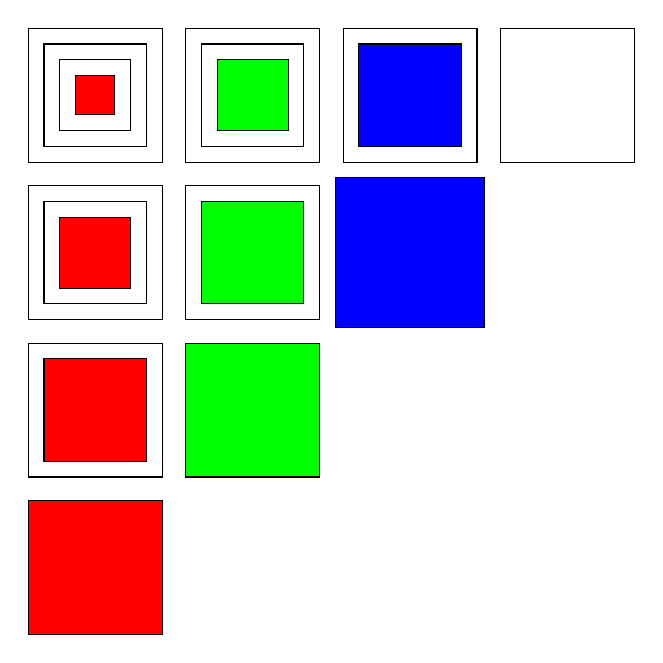
\begin{tikzpicture}[]
    \foreach \k [evaluate=\k as \s using {0.25+0.20*\k}] in {3, ..., 0} {
      \foreach \i [evaluate=\i as \m using {\k-\i}] in {0, ..., \k} {
        \foreach \j in {0, ..., \m} {
          \coordinate (C\i\j) at ($ 2*(\j,-\i) + (1.00cm,-1.00cm) $);
          \draw[draw=black] ($ (C\i\j) + (-\s,\s) $) rectangle ($ (C\i\j) + (\s,-\s) $);
        }
      }
    }

    \draw[fill=red] ($ (C00) + (-0.25, -0.25) $) rectangle ($ (C00) + (0.25, 0.25) $);
    \draw[fill=red] ($ (C10) + (-0.45, -0.45) $) rectangle ($ (C10) + (0.45, 0.45) $);
    \draw[fill=red] ($ (C20) + (-0.65, -0.65) $) rectangle ($ (C20) + (0.65, 0.65) $);
    \draw[fill=red] ($ (C30) + (-0.85, -0.85) $) rectangle ($ (C30) + (0.85, 0.85) $);

    \draw[fill=green] ($ (C01) + (-0.45, -0.45) $) rectangle ($ (C01) + (0.45, 0.45) $);
    \draw[fill=green] ($ (C11) + (-0.65, -0.65) $) rectangle ($ (C11) + (0.65, 0.65) $);
    \draw[fill=green] ($ (C21) + (-0.85, -0.85) $) rectangle ($ (C21) + (0.85, 0.85) $);

    \draw[fill=blue] ($ (C02) + (-0.65, -0.65) $) rectangle ($ (C02) + (0.65, 0.65) $);
    \draw[fill=blue] ($ (C12) + (-0.95, -0.95) $) rectangle ($ (C12) + (0.95, 0.95) $);

  \end{tikzpicture}
  \caption{Removing floor boxes from an~``ideal pyramid`` together with the
  boxes that depend on them. Order -- red, green, blue.}
  \label{fig:1CEGA}
\end{figure}
%%%%%%%%%%%%%%%%%%%%%%%%%%%%%%%%%%%%%%%%%%%%%%%%%%%%%%%%%%%%%%%%%%%%%%%%%%%%%%

In what follows, we'll construct a~``non-ideal pyramid``, consisting of $n$
boxes, by removing $r = m - n$ boxes from an ``ideal pyramid'' of size $k$
consisting of $m = Th(k)$. To see how much we can reduce the floor cost, when
removing total of $r$ boxes, we can just solve the quadratic equation
\eqref{eq:M2YJK} for $l$. The equation \eqref{eq:M2YJK} refactored to standard
form is
%%%%%%%%%%%%%%%%%%%%%%%%%%%%%%%%%%%%%%%%%%%%%%%%%%%%%%%%%%%%%%%%%%%%%%%%%%%%%%
\begin{equation}
  l^2 - (2k + 1) l  + 2 r = 0.
  \label{eq:Y0EY1}
\end{equation}
%%%%%%%%%%%%%%%%%%%%%%%%%%%%%%%%%%%%%%%%%%%%%%%%%%%%%%%%%%%%%%%%%%%%%%%%%%%%%%
The solution to~\eqref{eq:Y0EY1} is given by
%%%%%%%%%%%%%%%%%%%%%%%%%%%%%%%%%%%%%%%%%%%%%%%%%%%%%%%%%%%%%%%%%%%%%%%%%%%%%%
\begin{equation}
    \\
  \begin{aligned}
    & l = \frac{-b - \sqrt{b^2 - 8r}}{2}, & b = - (2 k + 1). &
  \end{aligned}
  \label{eq:NY9OF}
\end{equation}
%%%%%%%%%%%%%%%%%%%%%%%%%%%%%%%%%%%%%%%%%%%%%%%%%%%%%%%%%%%%%%%%%%%%%%%%%%%%%%
and finally the minimal number $f$ of boxes touching the floor for $n$ boxes in
total (i.e. the answer to the whole problem) is
%%%%%%%%%%%%%%%%%%%%%%%%%%%%%%%%%%%%%%%%%%%%%%%%%%%%%%%%%%%%%%%%%%%%%%%%%%%%%%
\begin{equation}
  f = f_k - \lfloor{l}\rfloor
 \label{eq:R6NHF}
\end{equation}
%%%%%%%%%%%%%%%%%%%%%%%%%%%%%%%%%%%%%%%%%%%%%%%%%%%%%%%%%%%%%%%%%%%%%%%%%%%%%%


\bibliographystyle{unsrtnat}
\bibliography{leetcode}

\end{document}

%% \label{??:BIW6X}
%% \label{??:N6ML4}
%% \label{??:R3UXE}
%% \label{??:X40DB}


% vim: set syntax=tex tabstop=2 shiftwidth=2 expandtab spell spelllang=en:
